\begin{refsection}

\def\chaptertitle{Background: The ecology, biodiversity, structure and function of southern African woodlands}


\chapter[\chaptertitle]{\chaptertitle}
\chaptermark{Background}
\label{ch:background}

\section{Introduction}
\label{background:sec:intro}

Tropical savannas are expected to experience significant shifts in vegetation structure and biodiversity in the coming century, due primarily to human induced climate change, land use change, and atmospheric carbon concentration \citep{Ross2021, Scheiter2009, Moncrieff2016}. Yet we lack a detailed understanding of how biodiversity and vegetation structure vary and affect ecosystem function (i.e. processes controlling fluxes of energy and matter through ecosystem across this highly heterogeneous biome, resulting in large uncertainty in earth system flux estimates across this biome \citep{Ahlstrom2015}. This thesis examines the role of tree species diversity as a driver of ecosystem function, with a focus on woody biomass and productivity as measures of ecosystem function, in southern African savannas. Biodiversity - Ecosystem Function (BEF) theory predicts positive effects of biodiversity on productivity \citep{Tilman2014}, but it is unclear whether this effect should occur in disturbance-prone and environmentally stressful ecosystems \citep{Steudel2012, Baert2018}. This chapter provides background on the ecology and biodiversity of tropical savannas and more specifically southern African woodlands, then summarises current literature on biodiversity-ecosystem function theory, to understand in greater depth the rationale for this thesis.

\section{The ecology of savannas}
\label{background:sec:savanna}

Savannas occupy \textapprox{}20\% of the global land surface \citep{Scholes1993}. They are the dominant land cover in the seasonal tropics, covering \textapprox{}40\% of the tropical land surface \citep{Scholes1997} (\autoref{background:savanna_map}). While debate continues around use of the term `savanna' \citep{Lehmann2011, Ratnam2011}, the generic definition used in this thesis characterises a savanna by the co-dominance of grass and trees, with a near contiguous grass-dominated understorey, and a closed or discontinuous, but sparse, woody overstorey \citep{Scholes1997, Bond2008}. Within this broad definition, savannas are highly heterogeneous, across local to continental scales \citep{Bucini2007}, with wide variation in canopy cover \citep{Sankaran2005, Hirota2011}, the functional and floristic composition of the woody overstorey \citep{Fayolle2018, Solbrig1996}, and the composition of the herbaceous understorey \citep{Siebert2019, Coller2018}.

Historically, tropical savannas were often mis-represented as severely degraded forests \citep{Veldman2016}. This view has roots in the nineteenth century idea of Clementsian succession and potential vegetation \citep{Pulsford2014}, which focussed on hierarchical physiognomic vegetation classifications with closed canopy forest at the top, rather than floristic or functional classifications that are in greater use at present \citep{Aleman2020}. The misinterpretation was exacerbated by the vast majority of early studies of savanna ecosystems originating from regions which lacked savanna vegetation. The hangover of this outdated paradigm is still felt today, with tropical savannas receiving less conservation funding \citep{Watson2016}, experiencing the greatest rates of transformation to agriculture of any major biome \citep{Hoekstra2004, Parr2014}, and being the focus of misplaced reforestation projects \citep{Silveira2020, Kumar2020, Laestadius2011}. In recent years there has been a push to acknowledge the value of tropical savannas, both intrinsically as centres of biodiversity and endemism \citep{Kumar2020, Pennington2018}, and as providers of ecosystem services \citep{Ryan2016}. Savannas proliferated globally during the Pliocene (\textapprox{}3-8 Mya), as a result of climate change, C4 grass proliferation, and an increase in the frequency and intensity of fire, with all three of these causes being inter-linked \citep{Cerling1997, Beerling2006, Edwards2010}. Rather than being viewed as derived landscapes that may be restored to a more forest-like environment, savannas should be considered a unique biome in their own right, with particular vegetation formations \citep{Torello2013}, a distinct evolutionary history \citep{Veldman2015}, and unique responses to global environmental change \citep{}.

\begin{figure}[!h]
\centering
	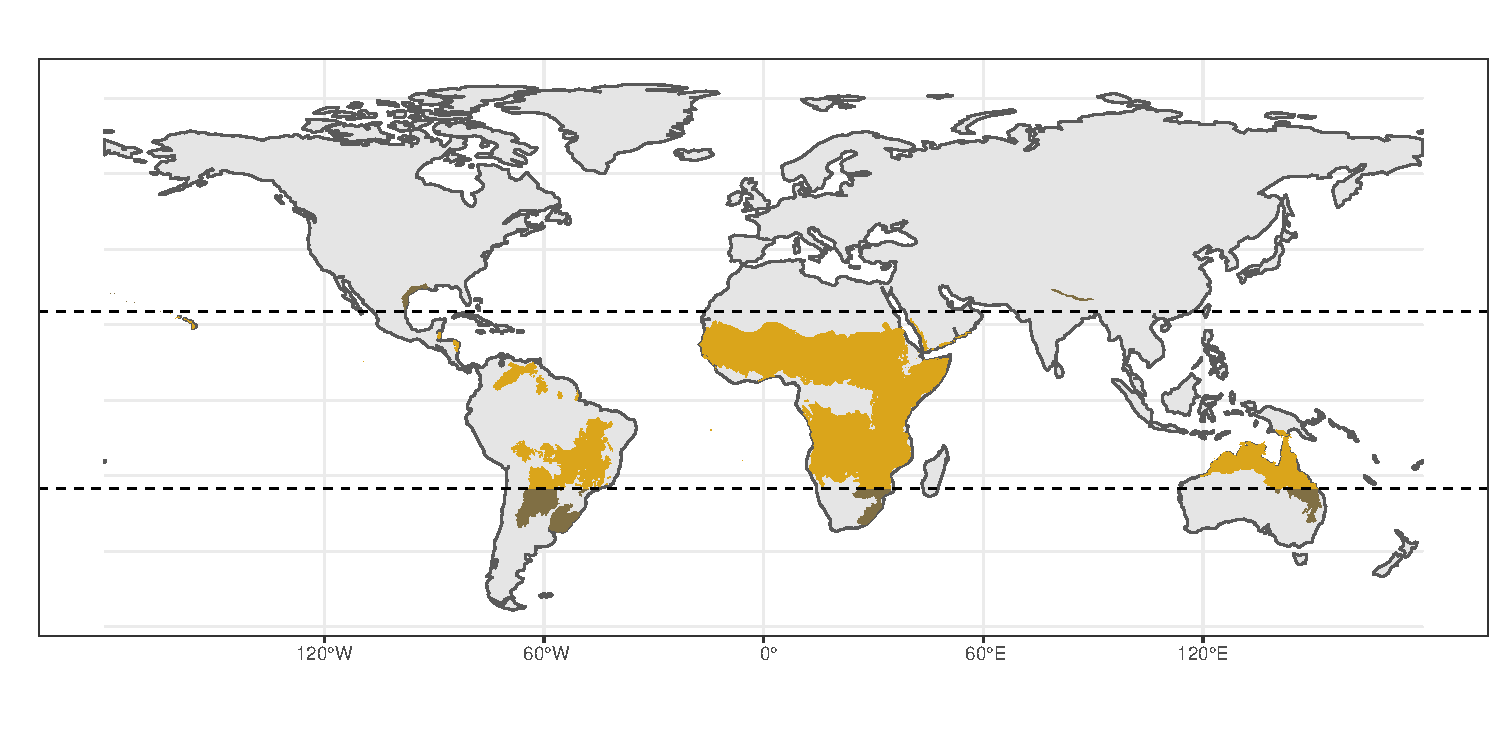
\includegraphics[width=\textwidth]{img/savanna_map}
	\caption[Map of global savanna distribution]{The global distribution of tropical savannas and grasslands (yellow), re-classified from the Terrestrial Ecoregions of the World \citep{Dinerstein2017}. Dashed lines mark the latitudinal extent of the tropics from N23.5\textdegree{} to S23.5\textdegree{}. Brown areas denote extra-tropical vegetation resembling tropical savannas.}
	\label{background:savanna_map}
\end{figure}

\subsection{Determinants of savanna vegetation}
\label{background:ssec:determ}

Savanna vegetation may occur as a result of multiple non-exclusive and interacting factors. One of the key questions in savanna ecology concerns identifying the factors driving variation in tree cover and assessing their relative importance in different contexts, thus determining the global distribution of savannas \citep{Higgins2000, Archibald2019}. Controls on tree cover can be split broadly into `disturbance-based' (e.g. fire, herbivory) or `resource-based' (e.g. precipitation, soil fertility)  \citep{Bond2008, Staver2015}. Both resource-based and disturbance-based controls on tree cover act simultaneously to varying extents in most savannas, though it is possible to classify savannas into two principal biomes based on their dominant control on tree cover, through their effects on species composition and woodland structure \citep{Huntley1982, Torello2013}. 

Tropical savannas occur in areas of high rainfall seasonality \citep{Lehmann2011}. At the continental scale, available moisture is the most significant determinant of savanna tree cover \citep{Sankaran2005}, setting the upper boundary of tree cover by physiological limitation of tree growth. In wetter mesic savannas, competition between grasses and trees is low, but in arid savannas, grasses may `poach' water from trees by intercepting it closer to the soil surface \citep{Scheiter2007}. While water availability may be the dominant resource-based determinant of savanna vegetation, edaphic properties also affect tree cover across savannas. Tropical savannas are often associated with nutrient-poor soils, especially in higher rainfall areas, where available nutrients are leached from the soil \citep{February2013}. Furthermore soil texture also interacts with rainfall to allow greater woody biomass and less grassy biomass where there is greater drainage \citep{Staver2011}. 

While resource availability, particularly moisture sets the upper bounds for tree cover, many savannas exist in areas that are climatically suitable for closed canopy forest \citep{Sankaran2005, Lehmann2011, Staver2011, Murphy2012}. Above \textapprox{}650 mm yr\textsuperscript{-1}, woody cover in savannas appears to show no dependence on MAP (\autoref{background:map_cover_plain}) \citep{Sankaran2008, Sankaran2005, Good2011}. In mesic savannas, where climatic conditions are suitable for closed canopy forest, there exists large heterogeneity in woody canopy cover at local spatial scales \citep{Dantas2015}. Mesic savannas often form a complex mosaic of open grassy patches and closed canopy forest-like patches, with their distribution dependent on local edaphic conditions and historical disturbance patterns \citep{Staver2011}. 

The key premise of the ``Alternative Stable States'' phenomenon is that contrasting ecosystem states may occur under similar environmental conditions, due to strong stabilising positive feedbacks on vegetation structure \citep{Staver2011}. Grass is the main fuel source for fires in mesic savannas. C\textsubscript{4} grasses, which dominate many mesic savannas, particularly in southern Africa \citep{Still2003}, are particularly flammable, but require more light than C3 grasses, meaning they are highly sensitive to variation in tree canopy cover \citep{CharlesDominique2018}. In areas with low grassy biomass, fire frequency and intensity are expected to be lower due to a lack of fuel. Simultaneously, juvenile trees are highly sensitive to fire in the grassy understorey layer due to their low stature, meaning that fire increases tree mortality, or `top-kill' of these individuals which must then resprout, keeping individuals small and creating a demographic bottleneck where only a few individuals grow to adults \citep{Bond1995, Ryan2011}. A positive feedback loop therefore occurs whereby disturbance by fire reduces canopy cover, allowing more frequent and intense fires, further reducing canopy cover as tree growth is suppressed. Alternatively, under reduced fire, trees can escape the `fire trap' in the understorey and grow to canopy trees \citep{Wakeling2011}, which rarely burn due to adaptive traits such as insulating bark and elevated crowns, increasing canopy cover, causing competitive exclusion of grasses \citep{Moustakas2013}, which further reduces disturbance by fire (\autoref{background:saf_theory}). 

\citet{Hirota2011}, using remotely sensed measures of tree cover across tropical Africa, South America and Australia, demonstrated a distinctly bi-modal distribution of tree cover within areas of intermediate rainfall (\textapprox{}650-1500 mm yr\textsuperscript{-1}). \citet{Staver2011} further showed that fire is the main source of this bi-modality. Furthermore, \citet{Staver2017} showed that change in fire return interval, whether the result of management or environmental change, can result in changes in ecosystem structure. Specifically, that longer fire return intervals result in a shift toward a more forest-like ecosystem with greater canopy closure, fewer small trees, and a greater number of large canopy trees.

\begin{figure}[!h]
\centering
	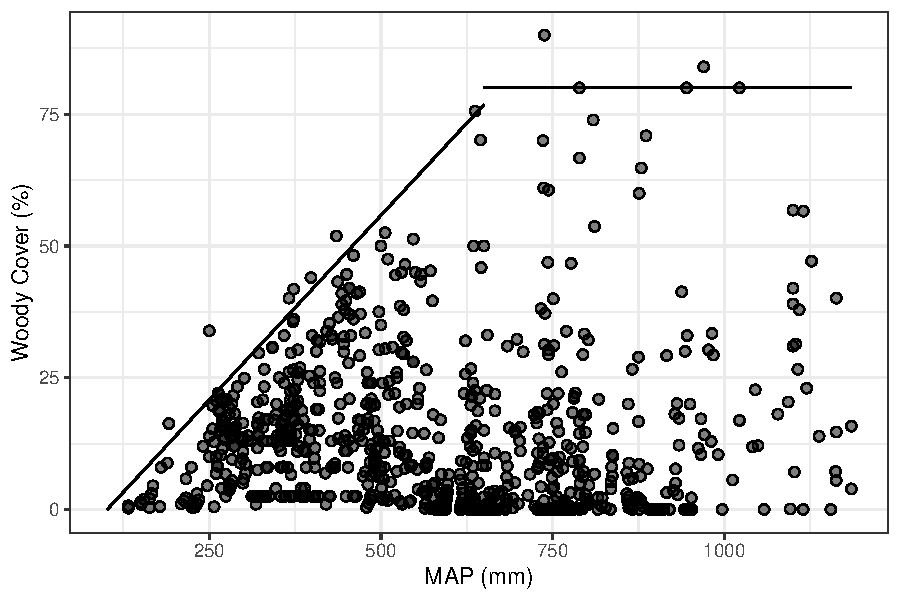
\includegraphics[width=\textwidth]{img/map_cover_plain}
	\caption[Precipitation vs. tree cover in southern Africa]{The relationship between rainfall (Mean Annual Precipitation) and proportional tree cover, across 854 savanna sites in Africa, adapted from \citet{Sankaran2005}. The line of best fit uses a broken-stick 99th quantile piece-wise linear regression to identify the breakpoint at which rainfall no longer sets the upper limit for tree cover. Above the breakpoint (650 $\pm$ 134 mm MAP) other processes such as disturbance by fire and local edaphic limitations are thought to determine tree cover.}
	\label{background:map_cover_plain}
\end{figure}

\begin{figure}[!h]
\centering
	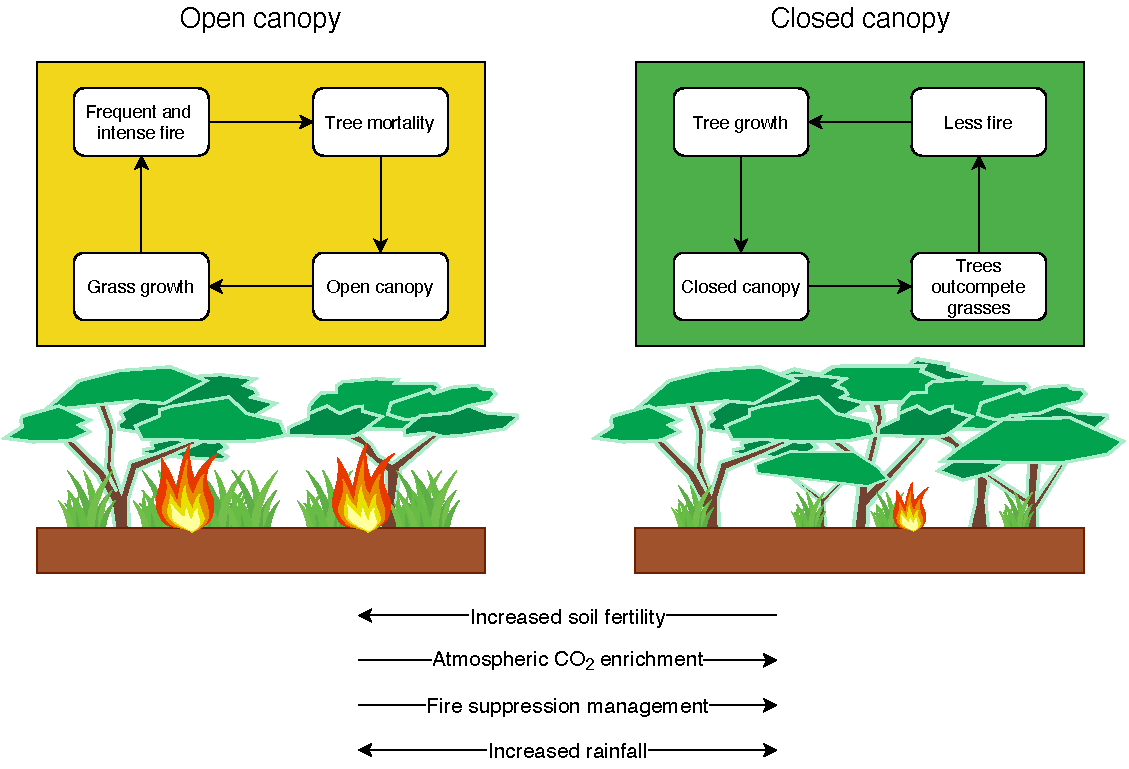
\includegraphics[width=\textwidth]{img/saf_theory}
	\caption[Schematic diagram of savanna positive feedback mechanisms]{The positive feedback mechanisms which determine the alternative stable states of mesic tropical savannas. Left: increased fire increases tree mortality, which decreases canopy cover, increasing available light for grass growth, leading to more fire and a further reduction in canopy cover. Right: decreased fire decreases tree mortality, which increases canopy cover, reducing available light to the grassy understorey, causing a reduction in grass fuel load, fewer fires and a further increase in canopy cover. Bottom: stabilising feedback loops can be disrupted given a large enough perturbation, causing a switch to another stable state. Some of these perturbations have different outcomes depending on the principal limitation of woody cover. In arid savannas, increased rainfall leads to an increase in woody cover, as more water percolates to deeper tree tap roots, while in a mesic savanna where water is not limiting, increased rainfall may lead to an increase in grass growth and therefore an increase in fire, which reduces woody cover.}
	\label{background:saf_theory}
\end{figure}

The factors described above which determine savanna vegetation structure are highly interactive. Moisture availability interacts with fire disturbance, leading, seemingly paradoxically, to a situation where increased resource availability may lead to lower woody biomass above a given threshold resource availability, due to increased grass growth and more intense and frequent fires \citep{Xu2015}. Soil nutrient availability also plays an interactive role with fire, increasing grass recovery rate between fires, which may lead to more frequent fires, increased tree mortality and lower woody biomass \citep{Kellman1984}. Interactions between environment, disturbance and tree cover, with clear thresholds of resource availability and tipping points of disturbance regime, result in a highly complex model of savanna ecosystem processes. 

\subsection{Adaptations of savanna trees}
\label{background:ssec:adapt}

Savanna trees are subject to a multitude of environmental pressures. To overcome these, savanna trees have a number of adaptations and employ various life history strategies, leading to a high functional diversity within tropical savanna trees \citep{Solbrig1996}, despite their low tree species diversity compared to tropical rainforests \citep{Solbrig1996}, for example.

Seasonal fires are a key determinant of savanna structure in mesic savannas (>650 mm MAP) \citep{Sankaran2005}. Many savanna tree species produce thick corky bark which protects the sapwood from high temperatures during fire \citep{Hoffmann2012, Lawes2011, Dantas2013}. Additionally, many savanna trees produce large below-ground root structures that are able to store carbohydrate, allowing individuals to re-sprout following fire \citep{Wigley2019}. There is evidence of adaptation in juveniles of some species that allows them to resprout in the same year following fire, giving them a head-start over competitors which adhere to a more rigid bud production cycle \citep{Wiegand2006}. Natural coppicing of adult savanna trees is common. If one growing tip is damaged due to fire, other stems on the same individual can continue growing, avoiding mortality. Savanna trees also sometimes have insulated buds to prevent fire reaching the sensitive growing tip \citep{CharlesDominique2015}.

Previously, root niche separation between grasses and trees was thought to be the main method by which trees and grasses coexist in savannas \citep{Walter1971}. Trees were observed to have deep tap roots while grasses have a greater density of fine near-surface roots \citep{Timberlake1993}. In arid savannas, root niche separation is an important mechanism allowing tree-grass coexistence, with consequences for the timing of seasonal growth in relation to seasonal rainfall intensity. In mesic savannas however, this effect is largely absent, except under specific edaphic conditions \citep{Case2020, Ketter2018, Sankaran2004, Higgins2000}. Recent work has shown that many savanna trees in mesic savannas produce two types of roots, the first are deep tap roots which are used primarily for water uptake and for storing carbohydrates as ligno-tubers to facilitate pre-rain green-up and resprouting following fire. The second are a mesh of finer roots which occur near to the surface and compete directly with grasses. These roots are used primarily for nutrient uptake, as most savanna soils have a distinct vertical nutrient profile \citep{Tomlinson2012, February2013}.  As an additional adaptation to overcome nutrient poor soils, many savanna trees readily produce root nodules with mutualistic \textit{Rhizobia} bacteria capable of fixing atmospheric nitrogen, or have ecto-mycorrhizal associations which improve phosphorus uptake \citep{Hogberg1986}. 

Fire removes much of the grass layer in a savanna, meaning that this is an ideal time for tree seedlings to germinate, as the lack of grass fuel means another fire is unlikely for some time, and the lack of grass cover means less competition for the growing seedling. Many tree species have adapted to having fire-activated seed dispersal \citep{Veldman2015}, with large seeds for long seed residence times, and rapid growth of newly emerged seedlings \citep{Daibes2019}, so that the seedlings can grow enough to escape the ``fire-trap'' before the grass fuel load has increased sufficiently to allow another fire. \citet{Wakeling2015} found that in densely grassy areas, a lack of gaps may prevent the germination of tree seeds, with long seed residence times allowing trees to take advantage of stochastic fire events that open up gaps for rooting. As an alternative to producing seed, many savanna trees reproduce predominantly via clonal growth. Clonal suckers remain connected to the natal tree, allowing rapid growth, as they benefit from the resources of the established carbohydrate-storing root structures \citep{Bond2003}.

Tropical savannas experience highly seasonal patterns of rainfall. Many savanna trees are deciduous, losing their leaves during the dry season to limit transpiration and conserve water \citep{Dahlin2016}. The phenomenon of `pre-rain green-up' has been observed widely across tropical savanna trees \citep{Archibald2007, Borchert1994, Williams1997}, whereby trees produce foliage material in advance of the rainy season. Multiple mechanisms have been suggested to explain pre-rain green-up as an adaptive trait, such as: to avoid competition for light and water \citep{Ryan2017}, to avoid herbivory \citep{Aide1988}, and to maximise the length of the growing season \citep{Scholes1993}. 

The many adaptations of savanna trees to disturbance and resource availability represent axes of functional variation which could lead to a greater contribution to ecosystem function under higher biodiversity. Specifically, greater resilience to disturbances and higher productivity maintained under seasonal variation in climate \citep{Diaz2001, Mori2012}.

\subsection{The global carbon cycle and change in savannas}
\label{background:ssec:carbon}

Tropical savannas contribute \textapprox{}30\% of global terrestrial Net Primary Productivity (NPP), i.e. atmospheric carbon fixed into biomass \citep{Grace2006}. Due to their large spatial extent, even a small percentage change in woody cover in savannas is expected to have large effects on the global carbon sink \citep{Williams2005}. Globally, savanna ecostystems are being degraded and lost to agricultural expansion, mining, and urban growth \citep{Parr2014}. \citet{Ross2021} predict biomass loss over most tropical savannas over the coming century, mostly due to land use change. Similarly, \citet{Aleman2016} concluded that land use change in sub-Saharan African savannas will have a greater negative effect on tree cover than changed in annual rainfall and rainfall seasonality. By 2100, the human population of sub-Saharan Africa is expected to double, increasing pressure on savanna ecosystems \citep{Pison2017}. Despite this, tropical savannas are reportedly the fastest increasing component of the terrestrial carbon sink \citep{Sitch2015}.

By 2050, it is expected that atmospheric CO\textsubscript{2} will have risen high enough that C\textsubscript{4} grasses no longer have a growth advantage over C\textsubscript{3} plants \citep{Bond2012}. An increase in atmospheric CO\textsubscript{2} is expected to lead to faster tree growth rates, allowing saplings to more quickly escape the ``fire-trap'', resulting in lower mortality, and a shift towards a closed canopy forest-like environment. Additionally, in arid savannas, the negative effect of CO\textsubscript{2} enrichment on grass transpiration rates \citep{Murphy2012} is expected to lead to less vigorous root growth and therefore more percolation of water to the deeper tree roots, increasing tree growth. 

Various studies, across the country of South Africa \citep{Stevens2016b}, the neotropics \citep{Rosan2019}, and globally \citep{Stevens2016}, have reported woody encroachment of trees into previously grassland or shrubland areas. However, due to the complex interactive nature of the determinants of savanna carbon cycling, it is still unclear whether these predicted effects of atmospheric CO\textsubscript{2} enrichment will materialise. \citet{Lewis2009} suggested that although existing woodlands are thickening, this does not necessarily extend to encroachment into previously unforested areas, due to the strong stabilising influence of fire. \citet{Pelletier2018} concluded that while more arid savannas will likely experience woody encroachment due primarily to the effects of CO\textsubscript{2} enrichment on transpiration and tree-grass water relations, there is no evidence that the same will happen in non-water limited savannas such as the miombo woodlands of southern Africa. Similarly, \citep{Reich2014} demonstrated that earth system models may be overly sensitive to the effects of CO\textsubscript{2} enrichment, and that the models suffer from a lack of mechanistic understanding of the effect of resource availability on disturbance. \citet{Korner2017} suggested that CO\textsubscript{2} enrichment may serve only to increase biomass turnover through increased growth offset by fire, with 44\% of all carbon emissions in savanna coming from fire \citep{Werf2010}, and 62\% of fire carbon emissions coming from savanna \citep{Werf2017}, offsetting the extra carbon sequestered.

Tropical savannas remain the largest source of uncertainty in models of the terrestrial carbon cycle \citep{Ahlstrom2015}. Environmental and land use change is expected to cause drastic changes to the functioning of savanna ecosystems in the coming century. Clearly, there is much work needed to better understand the interactive mechanisms which determine the role of tropical savannas in the global carbon cycle, and how these relations vary across environmental and biogeographic gradients. The wide functional diversity of savanna trees means that ecosystem level responses to global change will be complex, as adaptive traits determine varied individual responses, resulting likely in shifts in carbon storage and turnover of species in response to changes in rainfall, temperature, fire regime , and atmospheric carbon.

\section{Southern African woodlands}
\label{background:sec:southern_african}

This thesis focusses specifically on the mesic savannas of southern Africa, the savanna formations occurring in a latitudinal band south of the Congo basin rainforest, and north of the arid savannas of the country of South Africa (\autoref{background:saf_map}). These savannas cover approximately 2.7 million km\textsuperscript{2} \citep{Arino2010}. Hereafter they are referred to as southern African woodlands.

The structure of southern African woodlands is driven primarily by disturbance from fire and herbivory, leading to a highly heterogeneous patchy woodland habitat \citep{Archibald2019}. Fire return interval varies locally, dependent on climate and existing vegetation which determines grass fuel load \citep{Archibald2010}. Large herbivores play an important role in determining the vegetation structure of southern African woodlands. Compared to climatically similar savannas in the neotropics or southeast Asia, large herbivores are common in savannas throughout southern Africa \citep{Asner2009}. It has been suggested that large herbivores may cause disturbance in a manner similar to fires, reducing woody biomass by increasing mortality of juvenile saplings \citep{Bond2005}, though the effects of herbivory are often much more localised than fire, and the spatial distribution of herbivory cannot be predicted with the same detail \citep{Hempson2015}. While the dominant pressure determining the coexistence of grass and trees in savannas globally is moisture availability, within southern African woodlands where rainfall is rarely a limiting factor, competitiofor light is more important \citep{Vadigi2013}. Depending on the disturbance regime, southern African woodlands occassionally form dense closed canopies, while C\textsubscript{4} grasses are highly sensitive to shade. Feedbacks between tree cover and grass growth determine the fire regime and lead to highly heterogeneous woodland structure.

Southern African woodlands support a growing human population, with >150 million people benefitting from ecosystem services provided \citep{Ryan2016, Wunder2014}. Vast areas of woodland in southern Africa are used for grazing cattle which requires relatively open woodland \citep{Njana2013}, while other areas are used for charcoal production, bushmeat hunting, fruit, vegetable and mushroom foraging, and timber production \citep{Ryan2016}. Wood extraction by humans is increasing in southern Africa \citep{Hansen2013}, with more than 90\% of harvested wood used for energy production, mostly as charcoal in a domestic setting \citep{May-Tobin2011}. Other important ecosystem services provided by these woodlands to the human population include regulation of water availability throughout the dry season \citep{Wilk2010, Hecky2003} and the provision of medicinal plants \citep{Ryan2016, Augustino2011}. Simultaneously, southern African woodlands are inhabited by a high number of charismatic endemic species \citep{Burgess2004} and are increasingly a destination for international tourists \citep{Vergles2015, Shackleton2007}. These attributes together make southern African woodlands a hugely important natural asset, both locally and globally.

Southern African mesic savannas can be divided roughly into three dominant vegetation types. Miombo woodlands dominate southern Africa, and are the largest savanna vegetation type in the world \citep{Ryan2011}. They are dominated by species from the Fabaceae family, subfamily Detarioideae, from the genera: \textit{Brachystegia}, \textit{Julbernardia}, and \textit{Isoberlinia}, with the namesake `miombo' coming from the local name for the genus \textit{Brachystegia} in various Bantu languages. These woodlands frequently have tall continuous tree canopies that occassionally close to the point of excluding grasses, and are therefore frequently classified as forest by some forest cover maps \citep{Hansen2013}. Rainfall in miombo woodlands varies between 540-1700 mm yr\textsuperscript{-1}, with a highly seasonal pattern of precipitation. Miombo woodlands are highly diverse, with >8500 vascular plant species, of which >300 are tree species, many of which are endemic to the region \citep{Frost1996}.

Mopane woodlands form thin bands in the south of Zambia, Zimbabwe, central and southern Mozambique, and also across the border region of Angola and Namibia (\autoref{background:saf_map}). They are characterised by the dominance of a single tree species, \textit{Colophospermum mopane}, and generally occur in areas of lower rainfall than miombo woodlands \citep{Palgrave2003}. Reduced rainfall means that mopane soils are generally more fertile than the surrounding miombo woodlands \citep{Makhado2014}. Mopane woodlands are host to the largest diversity of large mammals in southern Africa, including populations of charismatic and highly threatened species such as the black rhinoceros (\textit{Diceros bicornis}) and giraffe (\textit{Giraffa camelopardalis}) \citep{Mittermeier2003}. While much of the mopane woodlands exists as short-stature shrubby vegetation, larger `cathedral mopane' exists in some areas, forming a near closed canopy \citep{Makhado2014}.

Baikiaea woodlands occur on sandy soils, in a wide belt along the Angolan-Namibian border to Zimbabwe. They are dominated by \textit{Baikiaea plurijuga}, which grow to large trees at low densities, with a grass and shrub understorey that burns regularly \citep{Werger1978}. Like \textit{C. mopane}, \textit{B. plurijuga} is also in the Detarioideae subfamily. Baikiaea woodlands are generally less suitable for agriculture than miombo woodlands, with highly sandy soil and low rainfall, though logging pressures have removed many of the largest and oldest trees in some regions \citep{}. Like mopane woodlands, Baikiaea woodlands provide habitat for many large herbivores \citep{}.

Although this thesis focusses primarily on the mesic savanna types described above, other savannas not dominated by large Detarioideae species also exist in southern Africa. Combretaceae woodlands are dominated by trees from the \textit{Combretum} and \textit{Terminalia}, both arbuscular mycorrhizal genera. Combretaceae woodlands are found in slightly drier but still dystrophic environmental conditions to miombo woodlands, but differ in their woodland structure, lacking large canopy tree species \citep{}. Finally, Mimosoideae woodlands occur in drier eurtrophic areas, often with higher levels of herbivory from large mammals than other woodlands in the region. Mimosoideae genera such as \textit{Acacia} often display `cagey' and thorny canopy architecture to protect from browsing mammals \citep{Maurin2014}. 

\begin{figure}[!h]
\centering
	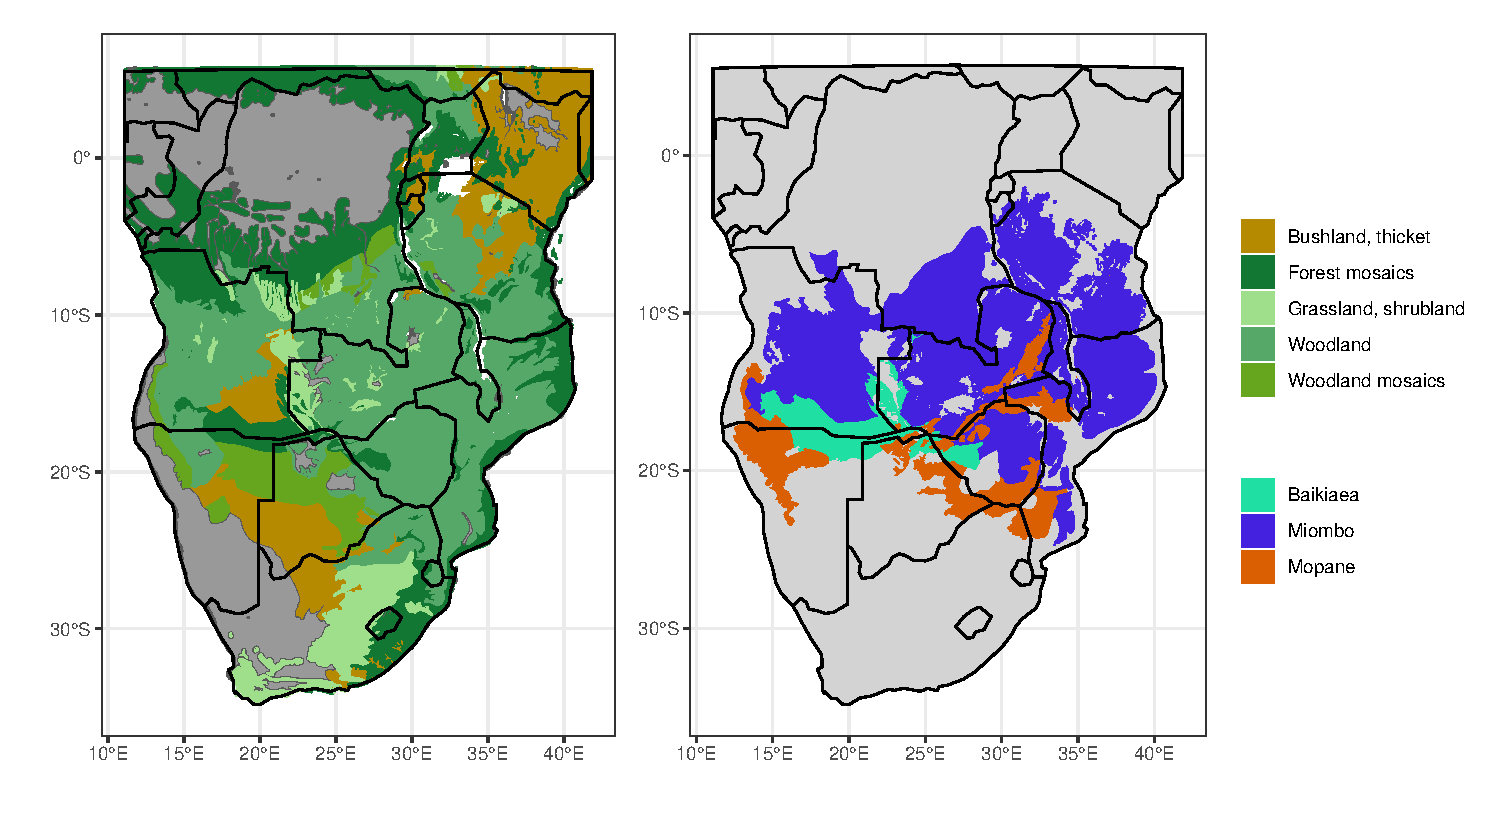
\includegraphics[width=\textwidth]{img/saf_map_both}
	\caption[Map of savanna vegetation types in Southern Africa]{The distribution of key savana vegetation types within southern Africa. Left: physiognomic classification adapted from \citet{White1983}. Right: floristic classification of selected savanna-woodlands adapted from \citet{Dinerstein2017}, Terrestrial Ecoregions of the World.}
	\label{background:saf_map}
\end{figure}

\section{Biodiversity and ecosystem function theory}
\label{background:sec:befr_theory}

In 1992, the Earth Summit in Rio de Janeiro discussed the growing concern that global patterns of biodiversity loss might negatively impact the functioning of ecosystems, and importantly damage the ecosystem services provided to humans. Later, researchers gathered in Bayreuth, Germany to discuss the role of biodiversity (B) on ecosystem function (EF) \citep{Schulze1993}. Since then, a thriving field of research has emerged which aims to assess and explain the multiple and complex relationships between biodiversity and ecosystem function (\autoref{background:befr_graph}), with hundreds of studies exploring biodiversity effects in both experimental and natural systems \citep{Plas2019, Newbold2016, Tilman2014}. The 1992 Earth Summit defined a paradigm shift in ecological thinking. Previously, biodiversity had mainly been considered a passive result of environmental conditions and ecosystem function, while the research that came after redefined biodiversity as both a driver and result of ecosystem function. BEF theory provides intuitive reasoning as to why increased biodiversity should lead to increased ecosystem function. 

BEF theory and supporting empirical evidence has informed global environmental policy by encouraging biodiversity conservation as a means of maintaining ecosystem functionality and its associated ecosystem services such as carbon storage, food provision, soil moisture retention etc. \citep{Balvanera2014, Naeem2012}. Increasingly, biodiversity conservation is being ecnouraged as a method of maximising natural capital (perceived value of natural assets, \citealt{Kareiva2011}) indirectly by maximising ecosystem functionality \citep{Scherer-Lorenzen2014, Cardinale2012}. Many conservation policy makers are seeking win-win conservation strategies which will maximise both biodiversity and ecosystem service provision \citep{Howe2014, Adams2004}. Research into the role of biodiversity in maintaining ecosystem functionality has become more pertinent in the last 20 years in response to mounting evidence of startling global biodiversity losses \citep{McRae2017, Butchart2010, Vitousek1997}. There is trepidation however, that as ecosystems are transformed as a result of conservation meant to maximise ecosystem function, or rather a subset of ecosystem functions that are easily measured and have been identified as valuable, such as carbon sequestration \citep{Duffy2017}, other ecosystem functions and services may suffer and the ecosystem may lose unique characteristics \citep{Brockerhoff2017, Srivastava2005a}. 

This thesis aims to understand variation in ecosystem function and community structure in southern African woodlands through the lens of the ``Biodiversity - Ecosystem Function Relationship'' (BEFR). Ecosystem functions can be defined in broad terms as the rate processes which control the fluxes of energy and matter through an ecosystem \citep{Jax2005}. This includes basic processes of primary production such as gross primary productivity and atmospheric nitrogen fixation, but can be extended to indirect aggregate measures of function such as resilience of productivity to disturbance. Additionally, ecosystem function can be further extended to ecosystem properties such as forest canopy complexity and trophic complexity, which in turn influence ecosystem processes. In this thesis, I focus only on biomass and productivity of trees as measures of ecosystem function, with the aim of improving our understanding of the carbon dynamics of southern African woodlands.

\begin{figure}[!h]
\centering
	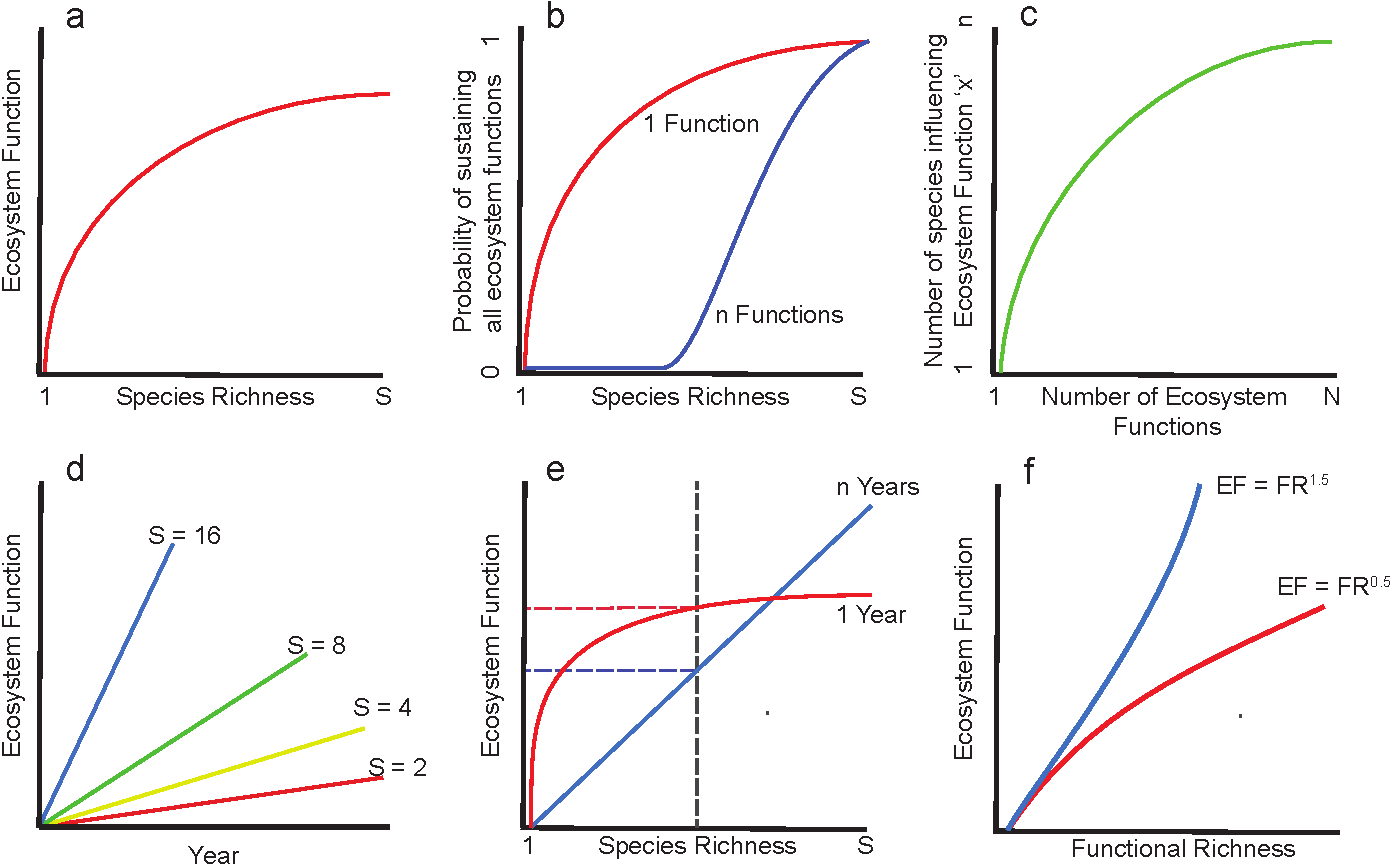
\includegraphics[width=\textwidth]{img/befr_graph}
	\caption[Inferences from previous Biodiversity-Ecosystem Function Research]{Schematic diagrams illustrating various inferences made on the Biodiversity - Ecosystem Function Relationship by previous studies. a) The classic BEF relationship found by many small scale experiments \citep{Cardinale2009}. b) As more functions are considered simultaneously the minimum species richness needed to maintain overall ecosystem functionality increases, also showing how the proportion of functionally redundant species increases as less functions are considered (i.e. the curve reaches asymptote at a lower species richness) \citep{Hector2007}. c) The saturating relationship of the number of ecosystem functions considered and the number of species influencing ecosystem multifunctionality \citep{Hector2007}. d) As studies progress through time the strength of the BEF relationhip increases, the rate of increase in ecosystem function increases as species richness (S) grows \citep{Cardinale2007}. e) As studies progress through time the shape of the relationship becomes more linear, saturating at progressively higher species richnesses. Studies averaged over longer periods exhibit a greater loss in ecosystem function in response to an equivalent species richness reduction \citep{Reich2012}. f) When functional richness is used in place of species richness, the relationship reaches asymptote at a higher richness. Additionally the relationship becomes more concave as a power coefficient representing the strength and number of species interactions increases. FR\textsuperscript{>1} (interspecific competition > intraspecific competition (unstable)) results in a convex relationship, while FR\textsuperscript{<1} results in a concave relationship \citep{Mora2014}.} 
	\label{background:befr_graph}
\end{figure}

\subsection{Niche complementarity, selection effects, and facilitation}
\label{background:ssec:niche}

% Selection effects
There are various mechanisms underlying the observed effect of biodiversity on ecosystem function. Early experiments in artificial grasslands \citep{Tilman1994} and experimental microcosms \citep{Naeem1994}, which involved introducing or removing species from random assemblages concluded that selection effects were the strongest drivers of the BEFR. Assuming random introduction or extinction of species, it is more likely that a diverse community will contain a species which contributes to a given ecosystem function \citep{Huston1997}. Of course, in natural systems, species introduction and removal is rarely random and may be confounded by a species' contribution to ecosystem functionality \citep{Smith2003}. Related to selection effects, which place emphasis on the presence of species which contribute to function, \citet{Grime1998} proposed the Mass-Ratio Hypothesis to explain biodiversity effects on ecosystem function. The Mass-Ratio Hypothesis suggests that it is not the breadth of niche space filled by a species assemblage that determines ecosystem functionality, but the ability of the most abundant species to optimise a chosen ecosystem function. Subsequent experimental studies have attempted to partition selection effects from other effects, or to remove selection effects entirely through experimental design, in an attempt to isolate other effects \citep{Loreau2001a}.

% Niche complementarity
The mechanism of niche complementarity has been the main focus of the majority of previous BEFR studies \citep{Wright2017} (\autoref{background:niche_all}). The theory of niche complementarity follows intuitively from early evolutionary theory, that coexisting species must occupy different environmental niches, in order to prevent competitive exclusion of the weaker competitor \citep{Tobner2016, Levine2009, MacArthur1955, MacArthur1967}. Thus, the more species present in a given system, the more environmental niche space is filled, leading to more efficient and complete use of resources, a reduction in density dependent intra-specific competition and `higher' observed values for various ecosystem functions \citep{Isbell2013}. The mechanism of niche complementarity has been corroborated by many studies, but to varying extents depending on biome, whether the study was conducted in an experimental or natural system, duration of study, and what measures of biodiversity and ecosystem function are used \citep{Wright2017, Cardinale2009, Cardinale2011}. Niche complementarity can also mediate functionality over time, as different species are able to optimise function at different times under under varying environmental conditions; this effect is known as the biodiversity insurance hypothesis \citep{Morin2014b, Bartomeus2013, Yachi1999a}. The insurance hypothesis also postulates that higher biodiversity at the landscape level will increase the rate at which ecosystems recover from stochastic local disturbances, by providing refugia populations in less perturbed areas \citep{Gonzalez2009}. 

% Facilitation
Facilitation effects increase the functional contribution of certain species in combination. For example, if grass species A is sensitive to high temperatures, tree species B may provide shade and thus reduce the temperature of the understorey, increasing the productivity of grass species A compared to if it was found in monoculture. Originally this specific example of facilitation was termed ``nurse plant syndrome'' \citep{Padilla2006}. This effect has been studied extensively in dryland ecosystems, where adult trees act as nurse plants for juveniles below, providing shade and reducing mortality. \citet{Callaway1997, Good2014, Weltzin1999} theorised a predictable relationship between environmental stress and the nature of interactions among plants, hypothesising that facilitation effects override competitive effects in highly stressful environments. More recently, \citet{Lortie2021} conducted a meta-analysis of facilitation effects in arid shrublands, concluding that while shrubs do provide facilitative effects, the net effect of species diversity on shrub biomass turned weakly negative under high diversity, due to competitive effects. Facilitation effects remain understudied in the BEFR literature. A history of research into partitioning niche complementarity from selection effects in biodiversity experiments has largely ignored the role of facilitation effects, presumably because they are not expected to drive large scale variation in the BEFR between systems, and because they are often context specific and difficult to test for their presence in natural systems \citep{Wright2017}. \citet{Wright2021} discusses how facilitation effects may have been mistakenly identified as niche complementarity as a result of the simplistic partitioning method used in previous studies.

\begin{figure}[!h]
\centering
	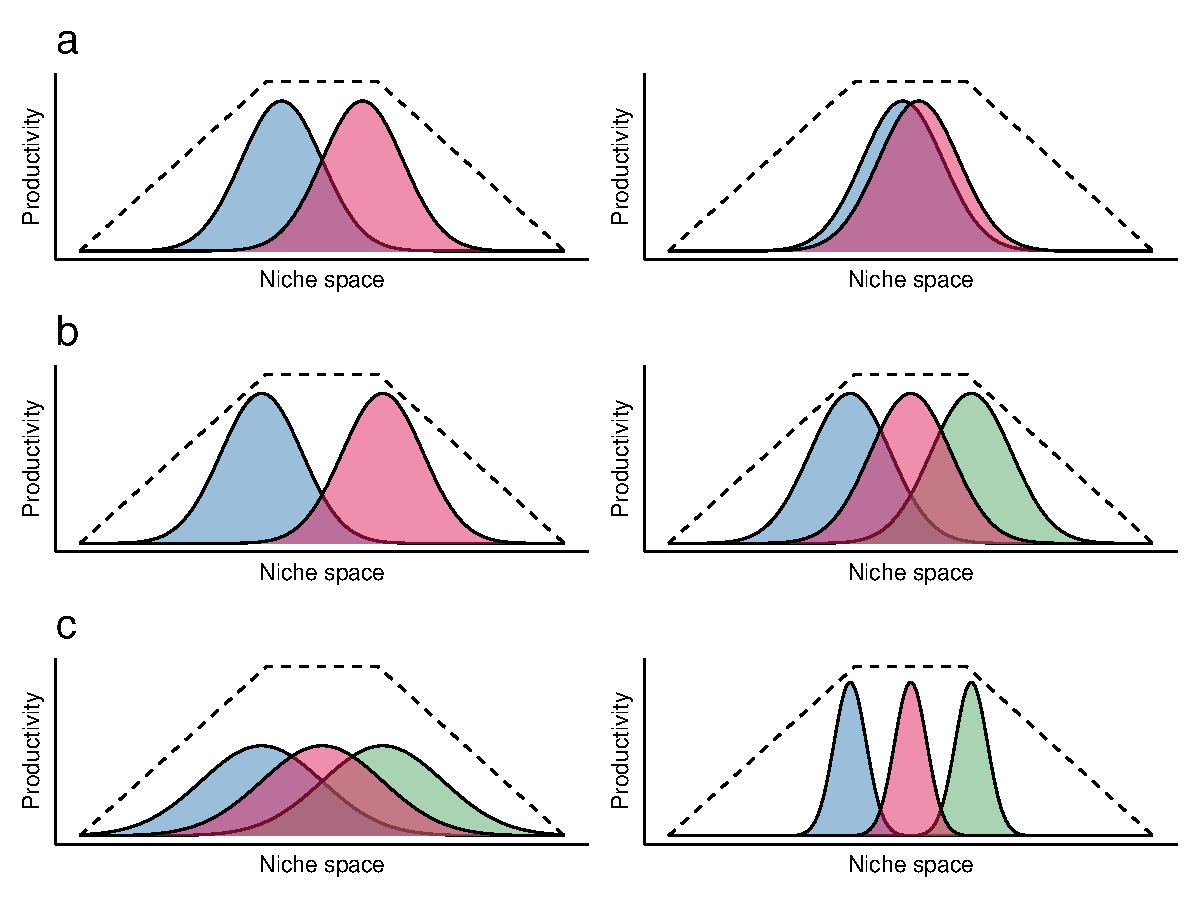
\includegraphics[width=\textwidth]{img/niche_all}
	\caption[Schematic diagrams demonstrating secondary controls on niche complementarity]{Schematic diagrams demonstrating niche occupation and secondary controls on the mechanism of niche complementarity. Each density plot shows a number of species, each represented by the species functional contribution (productivity) under different environmental conditions (niche space) within the larger environmental niche volume (dashed line). a) shows how the degree of overlap in functional niche of two species affects the total utilisation of the environmental niche volume (area under all species curves). When species are functionally distinct (left), more of the environmental niche volume is utilised. Removal of a species in this case would result in a large reduction in ecosystem productivity, while on the right, where functional redundancy is high, removal of a single species would have negligible effects. b) shows the effect of adding a functionally distinct species to an ecosystem. c) shows the effect of niche breadth on niche volume utilisation. On the left, three generalist species overlap in their functional niche. While each species has relatively incomplete utilisation of the environmental niche volume, this is offset as each species may occupy a wide range of environmental conditions. If the red species was removed, there would be only a marginal reduction in ecosystem productivity. On the right, three specialist species have a narrower niche breadth but a more complete utilisation of the environmental niche under ideal conditions. If a species was removed from this ecosystem, there would be a much greater reduction in ecosystem productivity.}
	\label{background:niche_all}
\end{figure}

\subsection{Global distribution of biodiversity-ecosystem function research}
\label{background:ssec:befr_global}

Among the hundreds of published studies of the biodiversity-ecosystem function relationship (BEFR), the majority are from experimental contexts, in small grassland patches or mesocosms. The number of studies in forested ecosystems is growing, but remains restricted predominantly to temperate forests in the global north \citep{Clarke2017}. In particular, there is a paucity of BEFR research in disturbance-prone wooded ecosystems, e.g. the mesic savannas which cover \textapprox{}20\% of the global land surface \citep{Scholes1993}. \citet{Liang2016} conducted a meta-analysis of estimates of the BEFR from 777,126 forest sample plots. They found that 99.87\% of these estimates followed a monotonic, positive BEFR curve, which saturated at high species richness. However, less than 600 of these plots were located in Africa, and none further south than Tanzania. 

\citet{Clarke2017} reviewed four BEFR meta-analyses \citep{Gamfeldt2015, Griffin2013a, Zhang2012, Cardinale2009} and identified only two studies conducted in Africa \citep{Foster1999, Burleigh1997}, compared with 69 in Europe and 82 in North America (\autoref{background:befr_map}). Both of these African studies are narrow in their scope and do not consider southern African woodland-savanna mosaics. \citet{Foster1999} studied the effect of dietary diversity on a single marine mollusc species in an experimental context. \citet{Burleigh1997} is an agroforestry study primarily investigating the suitability of two Fabaceae tree species as erosion mitigators. Neither of these studies provide an understanding of the BEFR that is relevant to understanding how entire savanna ecosystems respond to changes in biodiversity. In \citeauthor{Duffy2017}'s \citeyearpar{Duffy2017} meta-analysis, only three terrestial field studies from southern Africa were used to compare the effects of biodiversity to those of environmental factors from a total of 167 field estimates of the BEFR. Given the unique community composition \citep{Lehmann2011}, environmental conditions \citep{Linder2003} and strong role of disturbance by fire and herbivory in structuring these savannas, it would be unfeasible to generalise the BEFR found in other systems to this region.

\begin{figure}[!h]
\centering
	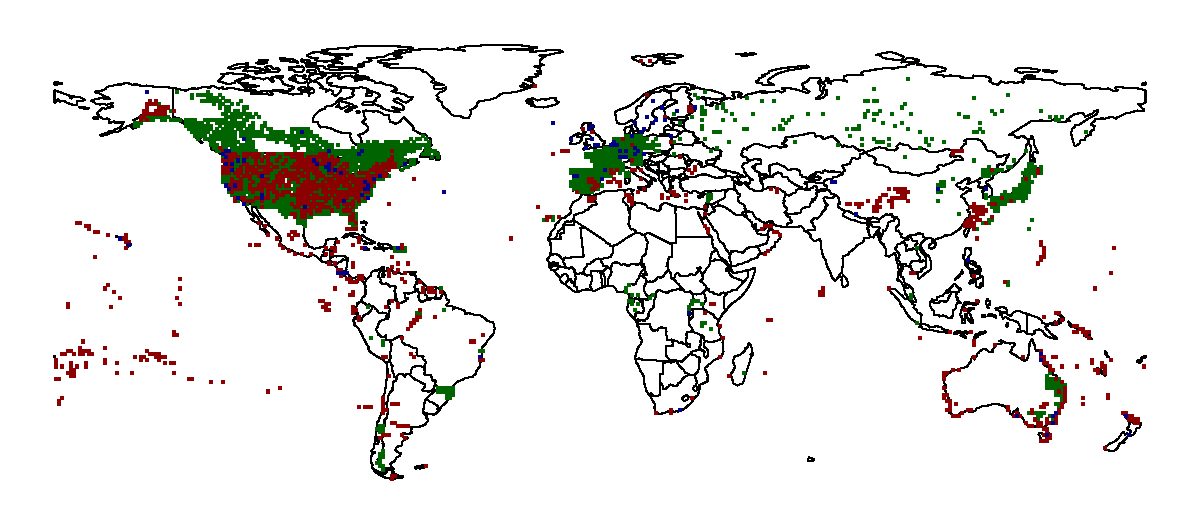
\includegraphics[width=\textwidth]{img/befr_map}
	\caption[Global distribution of Biodiversity-Ecosystem Function Relationship studies]{Location of studies of the biodiversity - ecosystem function relationship included in three meta-analyses of BEF research: blue \citet{Clarke2017}, green \citet{Liang2016}, red \citet{Duffy2017} - 67 field studies.}
	\label{background:befr_map}
\end{figure}

\subsection{Should we expect biodiversity effects on ecosystem function in southern African woodlands?}
\label{background:ssec:befr_africa}

Extensive research has linked tree biodiversity to ecosystem function in temperate and tropical forests \citep{Liang2016}, but tropical savannas differ in the environmental pressures they experience, and in the mechanisms which determine ecosystem structure. Conclusions drawn from BEFR research conducted in forests cannot necessarily be directly applied to disturbance driven and resource limited systems. 

Despite the current trend in conservation strategy to maximise biodiversity under the assumption that it will ensure ecosystem functionality, it remains unclear how important the BEFR is in determining ecosystem functionality compared to environmental factors \citep{Tilman2014}. It is also unclear to what extent the BEFR itself varies over environmental and biogeographical gradients \citep{Scherer-Lorenzen2014}. Many observed biodiversity effects could potentially be better explained by variation in unmeasured environmental variables, with which biodiversity merely correlates. Plant biodiversity has been shown to increase in areas with climatic conditions conducive to growth \citep{Fischer2014, Bunker2005}, and it is clear that temperature and precipitation also have a direct role in determining ecosystem functions such as net primary productivity and woody biomass \citep{Urban2017, Michaletz2014}.

A strong positive BEFR may not exist in all landscapes, with previous experimental and field studies producing many contrasting results. \citet{Duffy2017} conducted a meta-analysis of 133 estimates of the BEFR from 67 studies, suggesting comparable effects of biodiversity and climate or nutrient availability, but this generalisation remains largely speculative, especially for regions with a paucity of data, such as southern Africa (\autoref{background:befr_map}). Resource availability and disturbance frequency/intensity have been identified as two environmental factors that modulate the effect that biodiversity has on ecosystem functionality \citep{Tilman2012a, Tilman2014, Hooper2012}. In European forests, \citet{Ratcliffe2017} found that the strength of the effect of tree species richness on many ecosystem functions increased as water availability decreased. They suggested that facilitation effects between species became stronger than competitive effects when resource availability was low, with strong facilitation effects being more likely at high species richness. Furthermore, \citet{Baert2018} reported that environmental stress shows a humped relationship with the strength of the BEFR, with the relationship being highest at intermediate levels of stress. They suggest an interplay between niche complementarity and selection effects at low environmental stress levels, which are often accompanied by greater levels of competition due to the lack of growth limitation, and higher facilitative effects at very high levels of environmental stress. These environmental factors, which remain unmeasured in many studies of the BEFR in natural systems may explain some of the variation in the observed strength of the BEFR. Conducting experiments across environmental gradients will improve understanding of how biodiversity effects interact with the environment to determine ecosystem functionality \citep{Turnbull2016, Tilman2014}. \citet{Cardinale2002} found that in an experimental mesocosm of caddisfly larvae, increased disturbance in the form of random individual mortality led to increased effects of species richness on productivity. They attributed this effect to a decrease in dominance of competitively superior but low productivity taxa. Fire disturbance in forests has been linked to abundance dependent mortality among smaller stems \citep{Roques2001}. A species with more small stems is more likely to experience mortality during a fire. There may therefore be a link between disturbance regime and the strength of the species richness - ecosystem function relationship in fire prone woodland ecosystems. Unlike the caddisfly larvae in \citet{Cardinale2002} however, tree species differ in their resilience to fire driven mortality, owing to adaptations such as corky bark \citep{Solbrig1996}. The strength of the BEFR in a given system may therefore be a product of environmental conditions, disturbance regime, and species functional composition.

Biodiversity is often crudely measured as local species richness of a focal trophic level or functional group (e.g. trees). However, more complex measures such as functional richness provide better insight into the tangible organism level processes, which drive apparent species richness effects \citep{Finegan2015, Scherer-Lorenzen2014, Petchey2006}. For example, increased tree species richness appears to cause an increase in the productivity of forest stands, but is this due to there being a higher likelihood of having a productive species (selection effects), canopy packing complementarity, root depth complementarity, facilitative shading effects, or more likely a combination of all the above? It is likely that species richness is merely correlated with many other aspects of biodiversity which actually affect ecosystem function \citep{Mlambo2014, Scherer-Lorenzen2014}. Ultimately, there is no biological reason why two species should exhibit niche complementarity according to differences in species name. Of course, this is not to discount the role of phylogenetic and taxonomic separation as a proxy for degree of potential niche differentiation among species \citep{Flynn2011, Petchey2002}. Additionally, the distribution of relative contributions to a given function among species within an ecosystem is likely to affect the provision of that ecosystem function, through selection effects and the mass ratio hypothesis \citep{Chisholm2013b}. \textit{i.e.} a species with a high photosynthetic capacity will contribute little to overall ecosystem level productivity if it is found at very low abundances, but see \citet{Violle2017} and \citet{Soliveres2016}, which suggest that rare species often exhibit the least redundant traits and are therefore as functionally important as common species. Functional diversity should ideally be used to more directly quantify the functional contribution of species and individuals within an ecosystem, to understand better the mechanims that driver biodiversity effects.

In temperate and wet tropical closed canopy forests trees interact with each other due to their close proximity \citep{Coomes2007a, Purves2007}. Overlapping canopies and inter-weaving root networks produce competition for light, water and nutrients between individuals. Southern African woodlands however, exist along a wide gradient of tree cover. At the extreme low end of this gradient, trees are often too far apart for canopy competition to occur, and while the root networks of savanna trees are often extensive \citep{Belsky1994}, root competition may also approach zero between adult trees in the most sparsely wooded ecosystems. Low tree densities may result from a combination of ``resource-based'' processes such as low water availability and ``disturbance-based'' processes of disturbance caused by fire, herbivory, or human land use practices such as selective logging or tree felling for beehive harvesting \citep{Ryan2016}. \autoref{background:map_cover_plain} shows percentage woody cover along a precipitation gradient in Africa from \citet{Sankaran2005}. It shows that the majority of plots have a woody cover below the physiological maximum set by precipitation, indicating that many other factors influence woody cover other than water availability. A lack of competition would certainly weaken any effect of tree species diversity on ecosystem productivity, as multiple species can often fill overlapping niches in the absence of competition. Niche differentiation however, would still serve to only allow certain species to establish and optimise productivity in certain micro-habitats, suggesting at least some effect of tree diversity on ecosystem function even in the most sparsely forested ecosystems. Though \citet{Dohn2017} demonstrated strong competitive interactions at neighbourhood scales of up to 5 m for most trees in an East African savanna. Additionally, many savanna tree species do not grow well under shade \citep{Belsky1994}, unlike those in forests. Adult savanna trees will therefore compete with seedlings and saplings from their own species and from other species. Differences in competitive interactions amongst trees across tree cover gradients are likely to have an impact on the strength of the BEFR. 

\subsection{Demographic structure, structural diversity and ecosystem function}
\label{background:ssec:demography}

Disturbance by fire and herbivory, as well as drought and extreme temperature, create a bottleneck in the demographic structure of savannas, with high mortality of juveniles. The extent of this demographic bottleneck effect causes variation in tree canopy structure in different savannas. In the same way that co-existing tree species are expected to occupy different niche space to produce the positive niche complementarity effect on ecosystem function, it can be assumed that individuals occupying different demographic stages and with different canopy occupancy also opccupy different niche space. Thus, demographic and physical structure may represent a form of structural diversity that also influences ecosystem function.

In wet tropical forests \citep{} and temperate forests \citep{Danescu2016}, canopy layer diversity has been shown to increase productivity. Presumably an increase in canopy layer diversity 

\section{Conclusions}
\label{background:sec:conclusion}

Savannas are complex, and savanna vegetation arises as a result of many interacting factors. Tropical savannas are ecologically complex, but are understudied and represent the largest uncertainty in models of the global carbon cycle. Assumptions about the behaviour of tropical savannas cannot be made based on other tropical forested ecosystems, mainly due the pervasive role of disturbance and resource scarcity as drivers of ecosystem functioning. Previous studies of tropical savannas have focussed predominantly on the role of abiotic environment and disturbance as drivers of ecosystem function, with biodiversity as a passive result of these factors. Biodiversity - Ecosystem Function research reframes the role of biodiversity as both a driver and result of ecosystem function, and provides an intuitive prediction that biodiversity increases ecosystem function. However, BEF research in natural forested ecosystems has shown that both positive and negative biodiversity effects may occur, depending on the function studied and the intensity of environmental stress. It is unclear how biodiversity of tree species in southern African woodlands may affect productivity, but there are multiple reasons why biodiversity effects might be weaker or possibly negative in this biome. This thesis aims to increase our understanding of tree biodiversity in southern African woodlands, the world's largest savanna, through the lens of the Biodiversity-Ecosystem Function Relationship.

\newpage{}
\begingroup
\setstretch{1.0}
\printbibliography[heading=subbibintoc]
\endgroup

\end{refsection}

